%-*-latex-*-
\sectionthree{Insert}
\begin{python0}
from solutions import *; clear()
\end{python0}

Look at this maxheap again:

\begin{center}
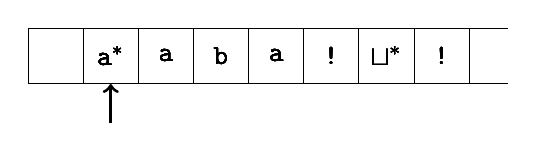
\begin{tikzpicture}

\draw (0.35, 0.35)
  node[draw, line width=0.01cm, , color=black,
       rounded corners=0cm, inner sep=0cm] {

\begin{minipage}[t][0.7cm]{0.7cm}
\mbox{}

\end{minipage}

};\draw (0.35, 0.35) node[color=black] {\texttt{\DOLLAR}};
\draw (1.0499999999999998, 0.35)
  node[draw, line width=0.01cm, , color=black,
       rounded corners=0cm, inner sep=0cm] {

\begin{minipage}[t][0.7cm]{0.7cm}
\mbox{}

\end{minipage}

};\draw (1.0499999999999998, 0.35) node[color=black] {\texttt{a$^*$}};
\draw (1.7499999999999998, 0.35)
  node[draw, line width=0.01cm, , color=black,
       rounded corners=0cm, inner sep=0cm] {

\begin{minipage}[t][0.7cm]{0.7cm}
\mbox{}

\end{minipage}

};\draw (1.7499999999999998, 0.35) node[color=black] {\texttt{a}};
\draw (2.4499999999999997, 0.35)
  node[draw, line width=0.01cm, , color=black,
       rounded corners=0cm, inner sep=0cm] {

\begin{minipage}[t][0.7cm]{0.7cm}
\mbox{}

\end{minipage}

};\draw (2.4499999999999997, 0.35) node[color=black] {\texttt{b}};
\draw (3.15, 0.35)
  node[draw, line width=0.01cm, , color=black,
       rounded corners=0cm, inner sep=0cm] {

\begin{minipage}[t][0.7cm]{0.7cm}
\mbox{}

\end{minipage}

};\draw (3.15, 0.35) node[color=black] {\texttt{a}};
\draw (3.85, 0.35)
  node[draw, line width=0.01cm, , color=black,
       rounded corners=0cm, inner sep=0cm] {

\begin{minipage}[t][0.7cm]{0.7cm}
\mbox{}

\end{minipage}

};\draw (3.85, 0.35) node[color=black] {\texttt{!}};
\draw (4.550000000000001, 0.35)
  node[draw, line width=0.01cm, , color=black,
       rounded corners=0cm, inner sep=0cm] {

\begin{minipage}[t][0.7cm]{0.7cm}
\mbox{}

\end{minipage}

};\draw (4.550000000000001, 0.35) node[color=black] {\texttt{$\sqcup^*$}};
\draw (5.25, 0.35)
  node[draw, line width=0.01cm, , color=black,
       rounded corners=0cm, inner sep=0cm] {

\begin{minipage}[t][0.7cm]{0.7cm}
\mbox{}

\end{minipage}

};\draw (5.25, 0.35) node[color=black] {\texttt{!}};
\draw (0.35, 0.35)
  node[draw, line width=0.01cm, , color=black,
       rounded corners=0cm, inner sep=0cm] {

\begin{minipage}[t][0.7cm]{0.7cm}
\mbox{}

\end{minipage}

};\draw (0.35, 0.35) node[color=black] {\texttt{\DOLLAR}};
\draw (1.0499999999999998, 0.35)
  node[draw, line width=0.01cm, , color=black,
       rounded corners=0cm, inner sep=0cm] {

\begin{minipage}[t][0.7cm]{0.7cm}
\mbox{}

\end{minipage}

};\draw (1.0499999999999998, 0.35) node[color=black] {\texttt{a$^*$}};
\draw (1.7499999999999998, 0.35)
  node[draw, line width=0.01cm, , color=black,
       rounded corners=0cm, inner sep=0cm] {

\begin{minipage}[t][0.7cm]{0.7cm}
\mbox{}

\end{minipage}

};\draw (1.7499999999999998, 0.35) node[color=black] {\texttt{a}};
\draw (2.4499999999999997, 0.35)
  node[draw, line width=0.01cm, , color=black,
       rounded corners=0cm, inner sep=0cm] {

\begin{minipage}[t][0.7cm]{0.7cm}
\mbox{}

\end{minipage}

};\draw (2.4499999999999997, 0.35) node[color=black] {\texttt{b}};
\draw (3.15, 0.35)
  node[draw, line width=0.01cm, , color=black,
       rounded corners=0cm, inner sep=0cm] {

\begin{minipage}[t][0.7cm]{0.7cm}
\mbox{}

\end{minipage}

};\draw (3.15, 0.35) node[color=black] {\texttt{a}};
\draw (3.85, 0.35)
  node[draw, line width=0.01cm, , color=black,
       rounded corners=0cm, inner sep=0cm] {

\begin{minipage}[t][0.7cm]{0.7cm}
\mbox{}

\end{minipage}

};\draw (3.85, 0.35) node[color=black] {\texttt{!}};
\draw (4.550000000000001, 0.35)
  node[draw, line width=0.01cm, , color=black,
       rounded corners=0cm, inner sep=0cm] {

\begin{minipage}[t][0.7cm]{0.7cm}
\mbox{}

\end{minipage}

};\draw (4.550000000000001, 0.35) node[color=black] {\texttt{$\sqcup^*$}};
\draw (5.25, 0.35)
  node[draw, line width=0.01cm, , color=black,
       rounded corners=0cm, inner sep=0cm] {

\begin{minipage}[t][0.7cm]{0.7cm}
\mbox{}

\end{minipage}

};\draw (5.25, 0.35) node[color=black] {\texttt{!}};
\draw (0.35, 0.35)
  node[draw, line width=0.01cm, , color=black,
       rounded corners=0cm, inner sep=0cm] {

\begin{minipage}[t][0.7cm]{0.7cm}
\mbox{}

\end{minipage}

};\draw (0.35, 0.35) node[color=black] {\texttt{\DOLLAR}};
\draw (1.0499999999999998, 0.35)
  node[draw, line width=0.01cm, , color=black,
       rounded corners=0cm, inner sep=0cm] {

\begin{minipage}[t][0.7cm]{0.7cm}
\mbox{}

\end{minipage}

};\draw (1.0499999999999998, 0.35) node[color=black] {\texttt{a$^*$}};
\draw (1.7499999999999998, 0.35)
  node[draw, line width=0.01cm, , color=black,
       rounded corners=0cm, inner sep=0cm] {

\begin{minipage}[t][0.7cm]{0.7cm}
\mbox{}

\end{minipage}

};\draw (1.7499999999999998, 0.35) node[color=black] {\texttt{a}};
\draw (2.4499999999999997, 0.35)
  node[draw, line width=0.01cm, , color=black,
       rounded corners=0cm, inner sep=0cm] {

\begin{minipage}[t][0.7cm]{0.7cm}
\mbox{}

\end{minipage}

};\draw (2.4499999999999997, 0.35) node[color=black] {\texttt{b}};
\draw (3.15, 0.35)
  node[draw, line width=0.01cm, , color=black,
       rounded corners=0cm, inner sep=0cm] {

\begin{minipage}[t][0.7cm]{0.7cm}
\mbox{}

\end{minipage}

};\draw (3.15, 0.35) node[color=black] {\texttt{a}};
\draw (3.85, 0.35)
  node[draw, line width=0.01cm, , color=black,
       rounded corners=0cm, inner sep=0cm] {

\begin{minipage}[t][0.7cm]{0.7cm}
\mbox{}

\end{minipage}

};\draw (3.85, 0.35) node[color=black] {\texttt{!}};
\draw (4.550000000000001, 0.35)
  node[draw, line width=0.01cm, , color=black,
       rounded corners=0cm, inner sep=0cm] {

\begin{minipage}[t][0.7cm]{0.7cm}
\mbox{}

\end{minipage}

};\draw (4.550000000000001, 0.35) node[color=black] {\texttt{$\sqcup^*$}};
\draw (5.25, 0.35)
  node[draw, line width=0.01cm, , color=black,
       rounded corners=0cm, inner sep=0cm] {

\begin{minipage}[t][0.7cm]{0.7cm}
\mbox{}

\end{minipage}

};\draw (5.25, 0.35) node[color=black] {\texttt{!}};
\draw (0.35, 0.35)
  node[draw, line width=0.01cm, , color=black,
       rounded corners=0cm, inner sep=0cm] {

\begin{minipage}[t][0.7cm]{0.7cm}
\mbox{}

\end{minipage}

};\draw (0.35, 0.35) node[color=black] {\texttt{\DOLLAR}};
\draw (1.0499999999999998, 0.35)
  node[draw, line width=0.01cm, , color=black,
       rounded corners=0cm, inner sep=0cm] {

\begin{minipage}[t][0.7cm]{0.7cm}
\mbox{}

\end{minipage}

};\draw (1.0499999999999998, 0.35) node[color=black] {\texttt{a$^*$}};
\draw (1.7499999999999998, 0.35)
  node[draw, line width=0.01cm, , color=black,
       rounded corners=0cm, inner sep=0cm] {

\begin{minipage}[t][0.7cm]{0.7cm}
\mbox{}

\end{minipage}

};\draw (1.7499999999999998, 0.35) node[color=black] {\texttt{a}};
\draw (2.4499999999999997, 0.35)
  node[draw, line width=0.01cm, , color=black,
       rounded corners=0cm, inner sep=0cm] {

\begin{minipage}[t][0.7cm]{0.7cm}
\mbox{}

\end{minipage}

};\draw (2.4499999999999997, 0.35) node[color=black] {\texttt{b}};
\draw (3.15, 0.35)
  node[draw, line width=0.01cm, , color=black,
       rounded corners=0cm, inner sep=0cm] {

\begin{minipage}[t][0.7cm]{0.7cm}
\mbox{}

\end{minipage}

};\draw (3.15, 0.35) node[color=black] {\texttt{a}};
\draw (3.85, 0.35)
  node[draw, line width=0.01cm, , color=black,
       rounded corners=0cm, inner sep=0cm] {

\begin{minipage}[t][0.7cm]{0.7cm}
\mbox{}

\end{minipage}

};\draw (3.85, 0.35) node[color=black] {\texttt{!}};
\draw (4.550000000000001, 0.35)
  node[draw, line width=0.01cm, , color=black,
       rounded corners=0cm, inner sep=0cm] {

\begin{minipage}[t][0.7cm]{0.7cm}
\mbox{}

\end{minipage}

};\draw (4.550000000000001, 0.35) node[color=black] {\texttt{$\sqcup^*$}};
\draw (5.25, 0.35)
  node[draw, line width=0.01cm, , color=black,
       rounded corners=0cm, inner sep=0cm] {

\begin{minipage}[t][0.7cm]{0.7cm}
\mbox{}

\end{minipage}

};\draw (5.25, 0.35) node[color=black] {\texttt{!}};
\draw (0.35, 0.35)
  node[draw, line width=0.01cm, , color=black,
       rounded corners=0cm, inner sep=0cm] {

\begin{minipage}[t][0.7cm]{0.7cm}
\mbox{}

\end{minipage}

};\draw (0.35, 0.35) node[color=black] {\texttt{\DOLLAR}};
\draw (1.0499999999999998, 0.35)
  node[draw, line width=0.01cm, , color=black,
       rounded corners=0cm, inner sep=0cm] {

\begin{minipage}[t][0.7cm]{0.7cm}
\mbox{}

\end{minipage}

};\draw (1.0499999999999998, 0.35) node[color=black] {\texttt{a$^*$}};
\draw (1.7499999999999998, 0.35)
  node[draw, line width=0.01cm, , color=black,
       rounded corners=0cm, inner sep=0cm] {

\begin{minipage}[t][0.7cm]{0.7cm}
\mbox{}

\end{minipage}

};\draw (1.7499999999999998, 0.35) node[color=black] {\texttt{a}};
\draw (2.4499999999999997, 0.35)
  node[draw, line width=0.01cm, , color=black,
       rounded corners=0cm, inner sep=0cm] {

\begin{minipage}[t][0.7cm]{0.7cm}
\mbox{}

\end{minipage}

};\draw (2.4499999999999997, 0.35) node[color=black] {\texttt{b}};
\draw (3.15, 0.35)
  node[draw, line width=0.01cm, , color=black,
       rounded corners=0cm, inner sep=0cm] {

\begin{minipage}[t][0.7cm]{0.7cm}
\mbox{}

\end{minipage}

};\draw (3.15, 0.35) node[color=black] {\texttt{a}};
\draw (3.85, 0.35)
  node[draw, line width=0.01cm, , color=black,
       rounded corners=0cm, inner sep=0cm] {

\begin{minipage}[t][0.7cm]{0.7cm}
\mbox{}

\end{minipage}

};\draw (3.85, 0.35) node[color=black] {\texttt{!}};
\draw (4.550000000000001, 0.35)
  node[draw, line width=0.01cm, , color=black,
       rounded corners=0cm, inner sep=0cm] {

\begin{minipage}[t][0.7cm]{0.7cm}
\mbox{}

\end{minipage}

};\draw (4.550000000000001, 0.35) node[color=black] {\texttt{$\sqcup^*$}};
\draw (5.25, 0.35)
  node[draw, line width=0.01cm, , color=black,
       rounded corners=0cm, inner sep=0cm] {

\begin{minipage}[t][0.7cm]{0.7cm}
\mbox{}

\end{minipage}

};\draw (5.25, 0.35) node[color=black] {\texttt{!}};
\draw (0.35, 0.35)
  node[draw, line width=0.01cm, , color=black,
       rounded corners=0cm, inner sep=0cm] {

\begin{minipage}[t][0.7cm]{0.7cm}
\mbox{}

\end{minipage}

};\draw (0.35, 0.35) node[color=black] {\texttt{\DOLLAR}};
\draw (1.0499999999999998, 0.35)
  node[draw, line width=0.01cm, , color=black,
       rounded corners=0cm, inner sep=0cm] {

\begin{minipage}[t][0.7cm]{0.7cm}
\mbox{}

\end{minipage}

};\draw (1.0499999999999998, 0.35) node[color=black] {\texttt{a$^*$}};
\draw (1.7499999999999998, 0.35)
  node[draw, line width=0.01cm, , color=black,
       rounded corners=0cm, inner sep=0cm] {

\begin{minipage}[t][0.7cm]{0.7cm}
\mbox{}

\end{minipage}

};\draw (1.7499999999999998, 0.35) node[color=black] {\texttt{a}};
\draw (2.4499999999999997, 0.35)
  node[draw, line width=0.01cm, , color=black,
       rounded corners=0cm, inner sep=0cm] {

\begin{minipage}[t][0.7cm]{0.7cm}
\mbox{}

\end{minipage}

};\draw (2.4499999999999997, 0.35) node[color=black] {\texttt{b}};
\draw (3.15, 0.35)
  node[draw, line width=0.01cm, , color=black,
       rounded corners=0cm, inner sep=0cm] {

\begin{minipage}[t][0.7cm]{0.7cm}
\mbox{}

\end{minipage}

};\draw (3.15, 0.35) node[color=black] {\texttt{a}};
\draw (3.85, 0.35)
  node[draw, line width=0.01cm, , color=black,
       rounded corners=0cm, inner sep=0cm] {

\begin{minipage}[t][0.7cm]{0.7cm}
\mbox{}

\end{minipage}

};\draw (3.85, 0.35) node[color=black] {\texttt{!}};
\draw (4.550000000000001, 0.35)
  node[draw, line width=0.01cm, , color=black,
       rounded corners=0cm, inner sep=0cm] {

\begin{minipage}[t][0.7cm]{0.7cm}
\mbox{}

\end{minipage}

};\draw (4.550000000000001, 0.35) node[color=black] {\texttt{$\sqcup^*$}};
\draw (5.25, 0.35)
  node[draw, line width=0.01cm, , color=black,
       rounded corners=0cm, inner sep=0cm] {

\begin{minipage}[t][0.7cm]{0.7cm}
\mbox{}

\end{minipage}

};\draw (5.25, 0.35) node[color=black] {\texttt{!}};
\draw (0.35, 0.35)
  node[draw, line width=0.01cm, , color=black,
       rounded corners=0cm, inner sep=0cm] {

\begin{minipage}[t][0.7cm]{0.7cm}
\mbox{}

\end{minipage}

};\draw (0.35, 0.35) node[color=black] {\texttt{\DOLLAR}};
\draw (1.0499999999999998, 0.35)
  node[draw, line width=0.01cm, , color=black,
       rounded corners=0cm, inner sep=0cm] {

\begin{minipage}[t][0.7cm]{0.7cm}
\mbox{}

\end{minipage}

};\draw (1.0499999999999998, 0.35) node[color=black] {\texttt{a$^*$}};
\draw (1.7499999999999998, 0.35)
  node[draw, line width=0.01cm, , color=black,
       rounded corners=0cm, inner sep=0cm] {

\begin{minipage}[t][0.7cm]{0.7cm}
\mbox{}

\end{minipage}

};\draw (1.7499999999999998, 0.35) node[color=black] {\texttt{a}};
\draw (2.4499999999999997, 0.35)
  node[draw, line width=0.01cm, , color=black,
       rounded corners=0cm, inner sep=0cm] {

\begin{minipage}[t][0.7cm]{0.7cm}
\mbox{}

\end{minipage}

};\draw (2.4499999999999997, 0.35) node[color=black] {\texttt{b}};
\draw (3.15, 0.35)
  node[draw, line width=0.01cm, , color=black,
       rounded corners=0cm, inner sep=0cm] {

\begin{minipage}[t][0.7cm]{0.7cm}
\mbox{}

\end{minipage}

};\draw (3.15, 0.35) node[color=black] {\texttt{a}};
\draw (3.85, 0.35)
  node[draw, line width=0.01cm, , color=black,
       rounded corners=0cm, inner sep=0cm] {

\begin{minipage}[t][0.7cm]{0.7cm}
\mbox{}

\end{minipage}

};\draw (3.85, 0.35) node[color=black] {\texttt{!}};
\draw (4.550000000000001, 0.35)
  node[draw, line width=0.01cm, , color=black,
       rounded corners=0cm, inner sep=0cm] {

\begin{minipage}[t][0.7cm]{0.7cm}
\mbox{}

\end{minipage}

};\draw (4.550000000000001, 0.35) node[color=black] {\texttt{$\sqcup^*$}};
\draw (5.25, 0.35)
  node[draw, line width=0.01cm, , color=black,
       rounded corners=0cm, inner sep=0cm] {

\begin{minipage}[t][0.7cm]{0.7cm}
\mbox{}

\end{minipage}

};\draw (5.25, 0.35) node[color=black] {\texttt{!}};
\draw (0.35, 0.35)
  node[draw, line width=0.01cm, , color=black,
       rounded corners=0cm, inner sep=0cm] {

\begin{minipage}[t][0.7cm]{0.7cm}
\mbox{}

\end{minipage}

};\draw (0.35, 0.35) node[color=black] {\texttt{\DOLLAR}};
\draw (1.0499999999999998, 0.35)
  node[draw, line width=0.01cm, , color=black,
       rounded corners=0cm, inner sep=0cm] {

\begin{minipage}[t][0.7cm]{0.7cm}
\mbox{}

\end{minipage}

};\draw (1.0499999999999998, 0.35) node[color=black] {\texttt{a$^*$}};
\draw (1.7499999999999998, 0.35)
  node[draw, line width=0.01cm, , color=black,
       rounded corners=0cm, inner sep=0cm] {

\begin{minipage}[t][0.7cm]{0.7cm}
\mbox{}

\end{minipage}

};\draw (1.7499999999999998, 0.35) node[color=black] {\texttt{a}};
\draw (2.4499999999999997, 0.35)
  node[draw, line width=0.01cm, , color=black,
       rounded corners=0cm, inner sep=0cm] {

\begin{minipage}[t][0.7cm]{0.7cm}
\mbox{}

\end{minipage}

};\draw (2.4499999999999997, 0.35) node[color=black] {\texttt{b}};
\draw (3.15, 0.35)
  node[draw, line width=0.01cm, , color=black,
       rounded corners=0cm, inner sep=0cm] {

\begin{minipage}[t][0.7cm]{0.7cm}
\mbox{}

\end{minipage}

};\draw (3.15, 0.35) node[color=black] {\texttt{a}};
\draw (3.85, 0.35)
  node[draw, line width=0.01cm, , color=black,
       rounded corners=0cm, inner sep=0cm] {

\begin{minipage}[t][0.7cm]{0.7cm}
\mbox{}

\end{minipage}

};\draw (3.85, 0.35) node[color=black] {\texttt{!}};
\draw (4.550000000000001, 0.35)
  node[draw, line width=0.01cm, , color=black,
       rounded corners=0cm, inner sep=0cm] {

\begin{minipage}[t][0.7cm]{0.7cm}
\mbox{}

\end{minipage}

};\draw (4.550000000000001, 0.35) node[color=black] {\texttt{$\sqcup^*$}};
\draw (5.25, 0.35)
  node[draw, line width=0.01cm, , color=black,
       rounded corners=0cm, inner sep=0cm] {

\begin{minipage}[t][0.7cm]{0.7cm}
\mbox{}

\end{minipage}

};\draw (5.25, 0.35) node[color=black] {\texttt{!}};\draw[line width=0.01cm,black] (5.6000000000000005,0.7) to  (6.1000000000000005,0.7);
\draw[line width=0.01cm,black] (5.6000000000000005,0.0) to  (6.1000000000000005,0.0);
\draw[line width=0.04cm,black,->] (1.05,-0.51) to  (1.05,-0.01);
\end{tikzpicture}

\end{center}



Suppose I want to insert a \verb!3! into the above tree.
To maintain the shape of a heap, I have to do it here:

{\small \begin{console}[frame=single,fontsize=\small]
[student@localhost 350-hashtable] g++ main.cpp; ./a.out
hash of
42: 42
42: 42
-1: 18446744073709551615
3.14: 5464867211497793177
0.0: 6369015886390043782
'a': 97
true: 1
"hello world": 5577293430985752569
\end{console}
}


(Don't forget that heaps are implemented with arrays
and therefore I can find the available slots in the array
right away with the length variable of the array.)
In this case the tree becomes perfect.
It's also a maxheap.

But what if I want to add \verb!8! into the tree instead?
I can again put it at the same spot:

\begin{center}
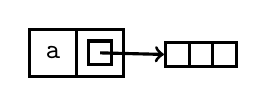
\begin{tikzpicture}

\draw (0.3, 0.3)
  node[draw, line width=0.04cm, , color=black,
       rounded corners=0cm, inner sep=0cm] {

\begin{minipage}[t][0.6cm]{0.6cm}
\mbox{}

\end{minipage}

};\draw (0.3, 0.3) node[color=black] {{\texttt{a}}};
\draw (0.8999999999999999, 0.3)
  node[draw, line width=0.04cm, , color=black,
       rounded corners=0cm, inner sep=0cm] {

\begin{minipage}[t][0.6cm]{0.6cm}
\mbox{}

\end{minipage}

};
\draw (0.9, 0.3)
  node[draw, line width=0.04cm, , color=black,
       rounded corners=0cm, inner sep=0cm] {

\begin{minipage}[t][0.3cm]{0.3cm}
\mbox{}

\end{minipage}

};
\draw (1.88, 0.28)
  node[draw, line width=0.04cm, , color=black,
       rounded corners=0cm, inner sep=0cm] {

\begin{minipage}[t][0.3cm]{0.3cm}
\mbox{}

\end{minipage}

};
\draw (2.1799999999999997, 0.28)
  node[draw, line width=0.04cm, , color=black,
       rounded corners=0cm, inner sep=0cm] {

\begin{minipage}[t][0.3cm]{0.3cm}
\mbox{}

\end{minipage}

};
\draw (2.48, 0.28)
  node[draw, line width=0.04cm, , color=black,
       rounded corners=0cm, inner sep=0cm] {

\begin{minipage}[t][0.3cm]{0.3cm}
\mbox{}

\end{minipage}

};\draw[line width=0.04cm,black,->] (0.9,0.3) to  (1.71,0.28);
\end{tikzpicture}

\end{center}



Of course this is not a maxheap any more.
What do I do?
I heapify-up.
I look at \verb!8!
and swap it with its parent if \verb!8! is larger than
its parent.
In this case, the parent is \verb!7!, so I swap them:

\begin{center}
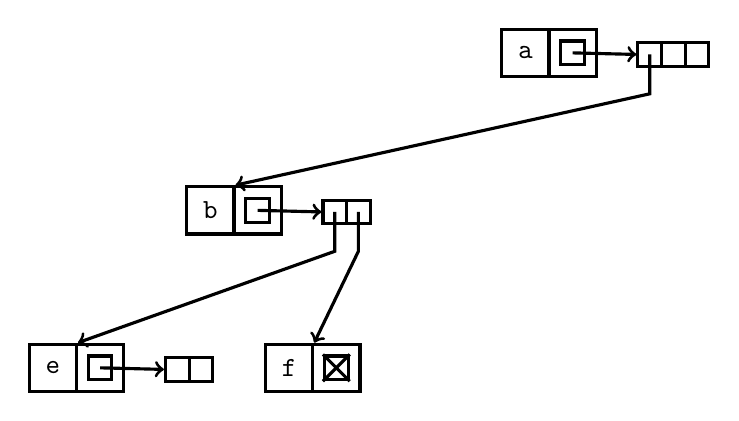
\begin{tikzpicture}

\draw (0.3, 0.3)
  node[draw, line width=0.04cm, , color=black,
       rounded corners=0cm, inner sep=0cm] {

\begin{minipage}[t][0.6cm]{0.6cm}
\mbox{}

\end{minipage}

};\draw (0.3, 0.3) node[color=black] {{\texttt{a}}};
\draw (0.8999999999999999, 0.3)
  node[draw, line width=0.04cm, , color=black,
       rounded corners=0cm, inner sep=0cm] {

\begin{minipage}[t][0.6cm]{0.6cm}
\mbox{}

\end{minipage}

};
\draw (0.9, 0.3)
  node[draw, line width=0.04cm, , color=black,
       rounded corners=0cm, inner sep=0cm] {

\begin{minipage}[t][0.3cm]{0.3cm}
\mbox{}

\end{minipage}

};
\draw (1.88, 0.28)
  node[draw, line width=0.04cm, , color=black,
       rounded corners=0cm, inner sep=0cm] {

\begin{minipage}[t][0.3cm]{0.3cm}
\mbox{}

\end{minipage}

};
\draw (2.1799999999999997, 0.28)
  node[draw, line width=0.04cm, , color=black,
       rounded corners=0cm, inner sep=0cm] {

\begin{minipage}[t][0.3cm]{0.3cm}
\mbox{}

\end{minipage}

};
\draw (2.48, 0.28)
  node[draw, line width=0.04cm, , color=black,
       rounded corners=0cm, inner sep=0cm] {

\begin{minipage}[t][0.3cm]{0.3cm}
\mbox{}

\end{minipage}

};\draw[line width=0.04cm,black,->] (0.9,0.3) to  (1.71,0.28);

\draw (-3.6999999999999997, -1.7)
  node[draw, line width=0.04cm, , color=black,
       rounded corners=0cm, inner sep=0cm] {

\begin{minipage}[t][0.6cm]{0.6cm}
\mbox{}

\end{minipage}

};\draw (-3.6999999999999997, -1.7) node[color=black] {{\texttt{b}}};
\draw (-3.0999999999999996, -1.7)
  node[draw, line width=0.04cm, , color=black,
       rounded corners=0cm, inner sep=0cm] {

\begin{minipage}[t][0.6cm]{0.6cm}
\mbox{}

\end{minipage}

};
\draw (-3.0999999999999996, -1.7)
  node[draw, line width=0.04cm, , color=black,
       rounded corners=0cm, inner sep=0cm] {

\begin{minipage}[t][0.3cm]{0.3cm}
\mbox{}

\end{minipage}

};
\draw (-2.12, -1.7200000000000002)
  node[draw, line width=0.04cm, , color=black,
       rounded corners=0cm, inner sep=0cm] {

\begin{minipage}[t][0.3cm]{0.3cm}
\mbox{}

\end{minipage}

};
\draw (-1.8199999999999998, -1.7200000000000002)
  node[draw, line width=0.04cm, , color=black,
       rounded corners=0cm, inner sep=0cm] {

\begin{minipage}[t][0.3cm]{0.3cm}
\mbox{}

\end{minipage}

};\draw[line width=0.04cm,black,->] (-3.1,-1.7) to  (-2.29,-1.72);

\draw (-5.7, -3.6999999999999997)
  node[draw, line width=0.04cm, , color=black,
       rounded corners=0cm, inner sep=0cm] {

\begin{minipage}[t][0.6cm]{0.6cm}
\mbox{}

\end{minipage}

};\draw (-5.7, -3.6999999999999997) node[color=black] {{\texttt{e}}};
\draw (-5.1, -3.6999999999999997)
  node[draw, line width=0.04cm, , color=black,
       rounded corners=0cm, inner sep=0cm] {

\begin{minipage}[t][0.6cm]{0.6cm}
\mbox{}

\end{minipage}

};
\draw (-5.1, -3.7)
  node[draw, line width=0.04cm, , color=black,
       rounded corners=0cm, inner sep=0cm] {

\begin{minipage}[t][0.3cm]{0.3cm}
\mbox{}

\end{minipage}

};
\draw (-4.119999999999999, -3.72)
  node[draw, line width=0.04cm, , color=black,
       rounded corners=0cm, inner sep=0cm] {

\begin{minipage}[t][0.3cm]{0.3cm}
\mbox{}

\end{minipage}

};
\draw (-3.8199999999999994, -3.72)
  node[draw, line width=0.04cm, , color=black,
       rounded corners=0cm, inner sep=0cm] {

\begin{minipage}[t][0.3cm]{0.3cm}
\mbox{}

\end{minipage}

};\draw[line width=0.04cm,black,->] (-5.1,-3.7) to  (-4.29,-3.72);

\draw (-2.7, -3.6999999999999997)
  node[draw, line width=0.04cm, , color=black,
       rounded corners=0cm, inner sep=0cm] {

\begin{minipage}[t][0.6cm]{0.6cm}
\mbox{}

\end{minipage}

};\draw (-2.7, -3.6999999999999997) node[color=black] {{\texttt{f}}};
\draw (-2.1, -3.6999999999999997)
  node[draw, line width=0.04cm, , color=black,
       rounded corners=0cm, inner sep=0cm] {

\begin{minipage}[t][0.6cm]{0.6cm}
\mbox{}

\end{minipage}

};
\draw (-2.1, -3.7)
  node[draw, line width=0.04cm, , color=black,
       rounded corners=0cm, inner sep=0cm] {

\begin{minipage}[t][0.3cm]{0.3cm}
\mbox{}

\end{minipage}

};\draw[line width=0.04cm,black] (-2.27,-3.53) to  (-1.93,-3.87);
\draw[line width=0.04cm,black] (-1.93,-3.53) to  (-2.27,-3.87);
\draw[line width=0.04cm,black,->] (1.88,0.28) to  (1.88,-0.22) to  (-3.38,-1.38);
\draw[line width=0.04cm,black,->] (-2.12,-1.72) to  (-2.12,-2.22) to  (-5.38,-3.38);
\draw[line width=0.04cm,black,->] (-1.82,-1.72) to  (-1.82,-2.22) to  (-2.38,-3.38);
\end{tikzpicture}

\end{center}



to get


\begin{center}
\begin{tikzpicture}[>=triangle 60,shorten >=0.5pt,node distance=2cm,auto,initial text=, double distance=2pt]
\node[state] (A) at (  0,  0) {$\{q_0\}$};
\node[state] (B) at (  3,  0) {$\{\}$};

\path[->]

;
\end{tikzpicture}
\end{center}
    


Now it's a maxheap again.
In general recall that heapify-up might involve
more than one swap.

In terms of the array implementation of the above heap, basically
this:


\begin{longtable}{|r||r|r|r|r|r|}
\hline 
         & $w_1$ & $w_2$ & $w_3$ & $w_4$ & $\ldots$ \\ \hline \hline 
$M_1$    &       &       &       &       &          \\ \hline 
$M_2$    &       &       &       &       &          \\ \hline 
$M_3$    &       &       &       &       &          \\ \hline 
$M_4$    &       &       &       &       &          \\ \hline 
$\ldots$ &       &       &       &       &          \\ \hline 
\end{longtable}
        


becomes this:


\begin{longtable}{|r||r|r|r|r|r|}
\hline 
         & $w_1$ & $w_2$ & $w_3$ & $w_4$ & $\ldots$ \\ \hline \hline 
$M_1$    & 0     & 0     & 1     & 0     & ...      \\ \hline 
$M_2$    & 1     & 0     & 1     & 1     & ...      \\ \hline 
$M_3$    & 0     & 1     & 1     & 1     & ...      \\ \hline 
$M_4$    & 1     & 0     & 1     & 1     & ...      \\ \hline 
$\ldots$ &       &       &       &       &          \\ \hline 
\end{longtable}
        


(Don't forget that technically speaking, there should also be a
length variable.)

Suppose I do this again: I add a \verb!9!.
It must go here:

\begin{center}
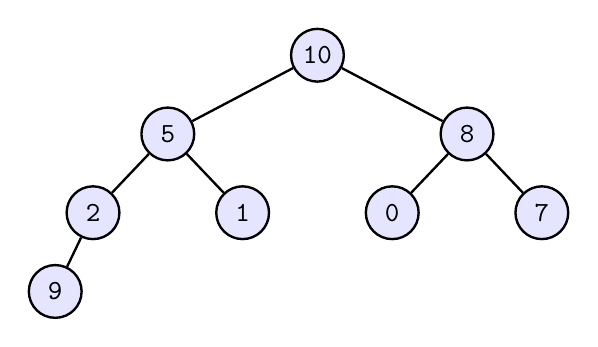
\begin{tikzpicture}

\fill[blue!10] (0.0, 0.0) circle (0.35);
\node [line width=0.03cm,black,minimum size=0.6699999999999999cm,draw,circle] at (0.0,0.0)(10){};\draw (0.0, 0.0) node[color=black] {\texttt{10}};
\fill[blue!10] (-1.9, -1.0) circle (0.35);
\node [line width=0.03cm,black,minimum size=0.6699999999999999cm,draw,circle] at (-1.9,-1.0)(5){};\draw (-1.9, -1.0) node[color=black] {\texttt{5}};
\fill[blue!10] (1.9, -1.0) circle (0.35);
\node [line width=0.03cm,black,minimum size=0.6699999999999999cm,draw,circle] at (1.9,-1.0)(8){};\draw (1.9, -1.0) node[color=black] {\texttt{8}};
\fill[blue!10] (-2.85, -2.0) circle (0.35);
\node [line width=0.03cm,black,minimum size=0.6699999999999999cm,draw,circle] at (-2.85,-2.0)(2){};\draw (-2.85, -2.0) node[color=black] {\texttt{2}};
\fill[blue!10] (-0.95, -2.0) circle (0.35);
\node [line width=0.03cm,black,minimum size=0.6699999999999999cm,draw,circle] at (-0.95,-2.0)(1){};\draw (-0.95, -2.0) node[color=black] {\texttt{1}};
\fill[blue!10] (0.95, -2.0) circle (0.35);
\node [line width=0.03cm,black,minimum size=0.6699999999999999cm,draw,circle] at (0.95,-2.0)(0){};\draw (0.95, -2.0) node[color=black] {\texttt{0}};
\fill[blue!10] (2.85, -2.0) circle (0.35);
\node [line width=0.03cm,black,minimum size=0.6699999999999999cm,draw,circle] at (2.85,-2.0)(7){};\draw (2.85, -2.0) node[color=black] {\texttt{7}};
\fill[blue!10] (-3.33, -3.0) circle (0.35);
\node [line width=0.03cm,black,minimum size=0.6699999999999999cm,draw,circle] at (-3.33,-3.0)(9){};\draw (-3.33, -3.0) node[color=black] {\texttt{9}};\draw[line width=0.03cm,black] (10) to  (5);
\draw[line width=0.03cm,black] (10) to  (8);
\draw[line width=0.03cm,black] (5) to  (2);
\draw[line width=0.03cm,black] (5) to  (1);
\draw[line width=0.03cm,black] (8) to  (0);
\draw[line width=0.03cm,black] (8) to  (7);
\draw[line width=0.03cm,black] (2) to  (9);
\end{tikzpicture}

\end{center}



(Draw the array implementation for the above.)
I swap \verb!9! and \verb!2! to get this:


\begin{center}
\begin{tikzpicture}[>=triangle 60,shorten >=0.5pt,node distance=2cm,auto,initial text=, double distance=2pt]
\node[state,initial] (A) at (  0,  0) {$\{q_0\}$};
\node[state] (B) at (  3,  0) {$\{\}$};

\path[->]
(A) edge [bend left=0,pos=0.5,above] node {$a,b$} (B)
(B) edge [loop above] node {$a,b$} ()

;
\end{tikzpicture}
\end{center}
    


and then swap \verb!9! and \verb!5! to get


\begin{center}
\begin{tikzpicture}[>=triangle 60,shorten >=0.5pt,node distance=2cm,auto,initial text=, double distance=2pt]
\node[state,initial] (A) at (  0,  0) {};

\path[->]
(A) edge [loop above] node {$a,b$} ()

;
\end{tikzpicture}
\end{center}
    


(Draw the arrays for the above so that you see how the array changes.)

This works even when you swap all the way to the root.
Say I add a \verb!20!.
It must go here:

\begin{console}[frame=single,fontsize=\footnotesize]
[student@localhost forward_list] g++ main.cpp; ./a.out
1.
true
size: 0
[3, 2, 1, 0]
[]
2.
[1, 2, 3, 4]
[2, 3, 4]
3.
[1, 2, 3, 4]
42
[42, 2, 3, 4]
4.
[1, 2, 3, 4]
[1, 2, 4]
5.
[1, 2, 3, 4]
[1, 2]
6.
[1, 2, 3, 4]
[1, 2, 77777, 88888, 99999, 3, 4]
7.
[1, 2, 3, 4]
[1, 2, -1, -1, -1, -1, -1, 3, 4]
8.
[1, 2, 3, 4]
[1, 2, 88, 99, 3, 4]
\end{console}



After 3 swaps I get:

\begin{console}[frame=single,fontsize=\footnotesize]
[student@localhost list] g++ main.cpp; ./a.out
1.
true
size: 0
[1, 0, 111, 222]
2.
[1, 2, 3, 4]
[2, 3]
3.
[1, 2, 3, 4]
[111, 2, 3, 999]
4.
[1, 2, 3, 4]
[1, 3, 4]
[1, 3, 4]
5.
[1, 2, 3, 4]
[1, 4]
6.
[1, 2, 3, 4]
[1, 99999, 88888, 77777, 2, 3, 4]
7.
[1, 2, 3, 4]
[1, -1, -1, -1, -1, -1, 2, 3, 4]
8.
[1, 2, 3, 4]
[1, 88, 99, 2, 3, 4]
9.
[1, 2, 3, 4]
4 3 2 1
\end{console}



and I get a maxheap again.

This process is called
\defterm{heapify-up}\tinysidebar{bubble-up \\ heapify-up \\ percolate up}
or
\defterm{bubble-up}
or
\defterm{percolate-up}.


\begin{ex} 
  \label{ex:some-decision1}
  \tinysidebar{\debug{exercises/{empty0/question.tex}}}
  \solutionlink{sol:some-decision1}
  \qed
\end{ex} 
\begin{python0}
from solutions import *
add(label="ex:some-decision1",
    srcfilename='exercises/some-decision1/answer.tex') 
\end{python0}

  
Now if you think about it,
if you have the following
\begin{center}
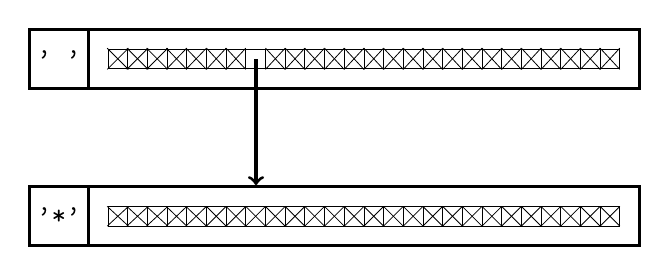
\begin{tikzpicture}

\draw (0.125, 0.125)
  node[draw, line width=0.01cm, , color=black,
       rounded corners=0cm, inner sep=0cm] {

\begin{minipage}[t][0.25cm]{0.25cm}
\mbox{}

\end{minipage}

};
\draw (0.375, 0.125)
  node[draw, line width=0.01cm, , color=black,
       rounded corners=0cm, inner sep=0cm] {

\begin{minipage}[t][0.25cm]{0.25cm}
\mbox{}

\end{minipage}

};
\draw (0.625, 0.125)
  node[draw, line width=0.01cm, , color=black,
       rounded corners=0cm, inner sep=0cm] {

\begin{minipage}[t][0.25cm]{0.25cm}
\mbox{}

\end{minipage}

};
\draw (0.875, 0.125)
  node[draw, line width=0.01cm, , color=black,
       rounded corners=0cm, inner sep=0cm] {

\begin{minipage}[t][0.25cm]{0.25cm}
\mbox{}

\end{minipage}

};
\draw (1.125, 0.125)
  node[draw, line width=0.01cm, , color=black,
       rounded corners=0cm, inner sep=0cm] {

\begin{minipage}[t][0.25cm]{0.25cm}
\mbox{}

\end{minipage}

};
\draw (1.375, 0.125)
  node[draw, line width=0.01cm, , color=black,
       rounded corners=0cm, inner sep=0cm] {

\begin{minipage}[t][0.25cm]{0.25cm}
\mbox{}

\end{minipage}

};
\draw (1.625, 0.125)
  node[draw, line width=0.01cm, , color=black,
       rounded corners=0cm, inner sep=0cm] {

\begin{minipage}[t][0.25cm]{0.25cm}
\mbox{}

\end{minipage}

};
\draw (1.875, 0.125)
  node[draw, line width=0.01cm, , color=black,
       rounded corners=0cm, inner sep=0cm] {

\begin{minipage}[t][0.25cm]{0.25cm}
\mbox{}

\end{minipage}

};
\draw (2.125, 0.125)
  node[draw, line width=0.01cm, , color=black,
       rounded corners=0cm, inner sep=0cm] {

\begin{minipage}[t][0.25cm]{0.25cm}
\mbox{}

\end{minipage}

};
\draw (2.375, 0.125)
  node[draw, line width=0.01cm, , color=black,
       rounded corners=0cm, inner sep=0cm] {

\begin{minipage}[t][0.25cm]{0.25cm}
\mbox{}

\end{minipage}

};
\draw (2.625, 0.125)
  node[draw, line width=0.01cm, , color=black,
       rounded corners=0cm, inner sep=0cm] {

\begin{minipage}[t][0.25cm]{0.25cm}
\mbox{}

\end{minipage}

};
\draw (2.875, 0.125)
  node[draw, line width=0.01cm, , color=black,
       rounded corners=0cm, inner sep=0cm] {

\begin{minipage}[t][0.25cm]{0.25cm}
\mbox{}

\end{minipage}

};
\draw (3.125, 0.125)
  node[draw, line width=0.01cm, , color=black,
       rounded corners=0cm, inner sep=0cm] {

\begin{minipage}[t][0.25cm]{0.25cm}
\mbox{}

\end{minipage}

};
\draw (3.375, 0.125)
  node[draw, line width=0.01cm, , color=black,
       rounded corners=0cm, inner sep=0cm] {

\begin{minipage}[t][0.25cm]{0.25cm}
\mbox{}

\end{minipage}

};
\draw (3.625, 0.125)
  node[draw, line width=0.01cm, , color=black,
       rounded corners=0cm, inner sep=0cm] {

\begin{minipage}[t][0.25cm]{0.25cm}
\mbox{}

\end{minipage}

};
\draw (3.875, 0.125)
  node[draw, line width=0.01cm, , color=black,
       rounded corners=0cm, inner sep=0cm] {

\begin{minipage}[t][0.25cm]{0.25cm}
\mbox{}

\end{minipage}

};
\draw (4.125, 0.125)
  node[draw, line width=0.01cm, , color=black,
       rounded corners=0cm, inner sep=0cm] {

\begin{minipage}[t][0.25cm]{0.25cm}
\mbox{}

\end{minipage}

};
\draw (4.375, 0.125)
  node[draw, line width=0.01cm, , color=black,
       rounded corners=0cm, inner sep=0cm] {

\begin{minipage}[t][0.25cm]{0.25cm}
\mbox{}

\end{minipage}

};
\draw (4.625, 0.125)
  node[draw, line width=0.01cm, , color=black,
       rounded corners=0cm, inner sep=0cm] {

\begin{minipage}[t][0.25cm]{0.25cm}
\mbox{}

\end{minipage}

};
\draw (4.875, 0.125)
  node[draw, line width=0.01cm, , color=black,
       rounded corners=0cm, inner sep=0cm] {

\begin{minipage}[t][0.25cm]{0.25cm}
\mbox{}

\end{minipage}

};
\draw (5.125, 0.125)
  node[draw, line width=0.01cm, , color=black,
       rounded corners=0cm, inner sep=0cm] {

\begin{minipage}[t][0.25cm]{0.25cm}
\mbox{}

\end{minipage}

};
\draw (5.375, 0.125)
  node[draw, line width=0.01cm, , color=black,
       rounded corners=0cm, inner sep=0cm] {

\begin{minipage}[t][0.25cm]{0.25cm}
\mbox{}

\end{minipage}

};
\draw (5.625, 0.125)
  node[draw, line width=0.01cm, , color=black,
       rounded corners=0cm, inner sep=0cm] {

\begin{minipage}[t][0.25cm]{0.25cm}
\mbox{}

\end{minipage}

};
\draw (5.875, 0.125)
  node[draw, line width=0.01cm, , color=black,
       rounded corners=0cm, inner sep=0cm] {

\begin{minipage}[t][0.25cm]{0.25cm}
\mbox{}

\end{minipage}

};
\draw (6.125, 0.125)
  node[draw, line width=0.01cm, , color=black,
       rounded corners=0cm, inner sep=0cm] {

\begin{minipage}[t][0.25cm]{0.25cm}
\mbox{}

\end{minipage}

};
\draw (6.375, 0.125)
  node[draw, line width=0.01cm, , color=black,
       rounded corners=0cm, inner sep=0cm] {

\begin{minipage}[t][0.25cm]{0.25cm}
\mbox{}

\end{minipage}

};
\draw (3.25, 0.125)
  node[draw, line width=0.04cm, , color=black,
       rounded corners=0cm, inner sep=0cm] {

\begin{minipage}[t][0.75cm]{7.0cm}
\mbox{}

\end{minipage}

};\draw[line width=0.01cm,black] (-0.01,0.26) to  (0.26,-0.01);
\draw[line width=0.01cm,black] (0.26,0.26) to  (-0.01,-0.01);
\draw[line width=0.01cm,black] (0.24,0.26) to  (0.51,-0.01);
\draw[line width=0.01cm,black] (0.51,0.26) to  (0.24,-0.01);
\draw[line width=0.01cm,black] (0.49,0.26) to  (0.76,-0.01);
\draw[line width=0.01cm,black] (0.76,0.26) to  (0.49,-0.01);
\draw[line width=0.01cm,black] (0.74,0.26) to  (1.0,-0.01);
\draw[line width=0.01cm,black] (1.0,0.26) to  (0.74,-0.01);
\draw[line width=0.01cm,black] (0.99,0.26) to  (1.25,-0.01);
\draw[line width=0.01cm,black] (1.25,0.26) to  (0.99,-0.01);
\draw[line width=0.01cm,black] (1.25,0.26) to  (1.5,-0.01);
\draw[line width=0.01cm,black] (1.5,0.26) to  (1.25,-0.01);
\draw[line width=0.01cm,black] (1.5,0.26) to  (1.75,-0.01);
\draw[line width=0.01cm,black] (1.75,0.26) to  (1.5,-0.01);
\draw[line width=0.01cm,black] (2.0,0.26) to  (2.25,-0.01);
\draw[line width=0.01cm,black] (2.25,0.26) to  (2.0,-0.01);
\draw[line width=0.01cm,black] (2.25,0.26) to  (2.5,-0.01);
\draw[line width=0.01cm,black] (2.5,0.26) to  (2.25,-0.01);
\draw[line width=0.01cm,black] (2.5,0.26) to  (2.75,-0.01);
\draw[line width=0.01cm,black] (2.75,0.26) to  (2.5,-0.01);
\draw[line width=0.01cm,black] (2.75,0.26) to  (3.0,-0.01);
\draw[line width=0.01cm,black] (3.0,0.26) to  (2.75,-0.01);
\draw[line width=0.01cm,black] (3.0,0.26) to  (3.25,-0.01);
\draw[line width=0.01cm,black] (3.25,0.26) to  (3.0,-0.01);
\draw[line width=0.01cm,black] (3.25,0.26) to  (3.5,-0.01);
\draw[line width=0.01cm,black] (3.5,0.26) to  (3.25,-0.01);
\draw[line width=0.01cm,black] (3.5,0.26) to  (3.75,-0.01);
\draw[line width=0.01cm,black] (3.75,0.26) to  (3.5,-0.01);
\draw[line width=0.01cm,black] (3.75,0.26) to  (4.0,-0.01);
\draw[line width=0.01cm,black] (4.0,0.26) to  (3.75,-0.01);
\draw[line width=0.01cm,black] (4.0,0.26) to  (4.25,-0.01);
\draw[line width=0.01cm,black] (4.25,0.26) to  (4.0,-0.01);
\draw[line width=0.01cm,black] (4.25,0.26) to  (4.5,-0.01);
\draw[line width=0.01cm,black] (4.5,0.26) to  (4.25,-0.01);
\draw[line width=0.01cm,black] (4.5,0.26) to  (4.75,-0.01);
\draw[line width=0.01cm,black] (4.75,0.26) to  (4.5,-0.01);
\draw[line width=0.01cm,black] (4.75,0.26) to  (5.0,-0.01);
\draw[line width=0.01cm,black] (5.0,0.26) to  (4.75,-0.01);
\draw[line width=0.01cm,black] (5.0,0.26) to  (5.25,-0.01);
\draw[line width=0.01cm,black] (5.25,0.26) to  (5.0,-0.01);
\draw[line width=0.01cm,black] (5.25,0.26) to  (5.5,-0.01);
\draw[line width=0.01cm,black] (5.5,0.26) to  (5.25,-0.01);
\draw[line width=0.01cm,black] (5.5,0.26) to  (5.75,-0.01);
\draw[line width=0.01cm,black] (5.75,0.26) to  (5.5,-0.01);
\draw[line width=0.01cm,black] (5.75,0.26) to  (6.0,-0.01);
\draw[line width=0.01cm,black] (6.0,0.26) to  (5.75,-0.01);
\draw[line width=0.01cm,black] (6.0,0.26) to  (6.25,-0.01);
\draw[line width=0.01cm,black] (6.25,0.26) to  (6.0,-0.01);
\draw[line width=0.01cm,black] (6.25,0.26) to  (6.5,-0.01);
\draw[line width=0.01cm,black] (6.5,0.26) to  (6.25,-0.01);

\draw (-0.625, 0.125)
  node[draw, line width=0.04cm, , color=black,
       rounded corners=0cm, inner sep=0cm] {

\begin{minipage}[t][0.75cm]{0.75cm}
\mbox{}

\end{minipage}

};\draw (-0.625, 0.125) node[color=black] {\texttt{' '}};
\draw (0.125, -1.875)
  node[draw, line width=0.01cm, , color=black,
       rounded corners=0cm, inner sep=0cm] {

\begin{minipage}[t][0.25cm]{0.25cm}
\mbox{}

\end{minipage}

};
\draw (0.375, -1.875)
  node[draw, line width=0.01cm, , color=black,
       rounded corners=0cm, inner sep=0cm] {

\begin{minipage}[t][0.25cm]{0.25cm}
\mbox{}

\end{minipage}

};
\draw (0.625, -1.875)
  node[draw, line width=0.01cm, , color=black,
       rounded corners=0cm, inner sep=0cm] {

\begin{minipage}[t][0.25cm]{0.25cm}
\mbox{}

\end{minipage}

};
\draw (0.875, -1.875)
  node[draw, line width=0.01cm, , color=black,
       rounded corners=0cm, inner sep=0cm] {

\begin{minipage}[t][0.25cm]{0.25cm}
\mbox{}

\end{minipage}

};
\draw (1.125, -1.875)
  node[draw, line width=0.01cm, , color=black,
       rounded corners=0cm, inner sep=0cm] {

\begin{minipage}[t][0.25cm]{0.25cm}
\mbox{}

\end{minipage}

};
\draw (1.375, -1.875)
  node[draw, line width=0.01cm, , color=black,
       rounded corners=0cm, inner sep=0cm] {

\begin{minipage}[t][0.25cm]{0.25cm}
\mbox{}

\end{minipage}

};
\draw (1.625, -1.875)
  node[draw, line width=0.01cm, , color=black,
       rounded corners=0cm, inner sep=0cm] {

\begin{minipage}[t][0.25cm]{0.25cm}
\mbox{}

\end{minipage}

};
\draw (1.875, -1.875)
  node[draw, line width=0.01cm, , color=black,
       rounded corners=0cm, inner sep=0cm] {

\begin{minipage}[t][0.25cm]{0.25cm}
\mbox{}

\end{minipage}

};
\draw (2.125, -1.875)
  node[draw, line width=0.01cm, , color=black,
       rounded corners=0cm, inner sep=0cm] {

\begin{minipage}[t][0.25cm]{0.25cm}
\mbox{}

\end{minipage}

};
\draw (2.375, -1.875)
  node[draw, line width=0.01cm, , color=black,
       rounded corners=0cm, inner sep=0cm] {

\begin{minipage}[t][0.25cm]{0.25cm}
\mbox{}

\end{minipage}

};
\draw (2.625, -1.875)
  node[draw, line width=0.01cm, , color=black,
       rounded corners=0cm, inner sep=0cm] {

\begin{minipage}[t][0.25cm]{0.25cm}
\mbox{}

\end{minipage}

};
\draw (2.875, -1.875)
  node[draw, line width=0.01cm, , color=black,
       rounded corners=0cm, inner sep=0cm] {

\begin{minipage}[t][0.25cm]{0.25cm}
\mbox{}

\end{minipage}

};
\draw (3.125, -1.875)
  node[draw, line width=0.01cm, , color=black,
       rounded corners=0cm, inner sep=0cm] {

\begin{minipage}[t][0.25cm]{0.25cm}
\mbox{}

\end{minipage}

};
\draw (3.375, -1.875)
  node[draw, line width=0.01cm, , color=black,
       rounded corners=0cm, inner sep=0cm] {

\begin{minipage}[t][0.25cm]{0.25cm}
\mbox{}

\end{minipage}

};
\draw (3.625, -1.875)
  node[draw, line width=0.01cm, , color=black,
       rounded corners=0cm, inner sep=0cm] {

\begin{minipage}[t][0.25cm]{0.25cm}
\mbox{}

\end{minipage}

};
\draw (3.875, -1.875)
  node[draw, line width=0.01cm, , color=black,
       rounded corners=0cm, inner sep=0cm] {

\begin{minipage}[t][0.25cm]{0.25cm}
\mbox{}

\end{minipage}

};
\draw (4.125, -1.875)
  node[draw, line width=0.01cm, , color=black,
       rounded corners=0cm, inner sep=0cm] {

\begin{minipage}[t][0.25cm]{0.25cm}
\mbox{}

\end{minipage}

};
\draw (4.375, -1.875)
  node[draw, line width=0.01cm, , color=black,
       rounded corners=0cm, inner sep=0cm] {

\begin{minipage}[t][0.25cm]{0.25cm}
\mbox{}

\end{minipage}

};
\draw (4.625, -1.875)
  node[draw, line width=0.01cm, , color=black,
       rounded corners=0cm, inner sep=0cm] {

\begin{minipage}[t][0.25cm]{0.25cm}
\mbox{}

\end{minipage}

};
\draw (4.875, -1.875)
  node[draw, line width=0.01cm, , color=black,
       rounded corners=0cm, inner sep=0cm] {

\begin{minipage}[t][0.25cm]{0.25cm}
\mbox{}

\end{minipage}

};
\draw (5.125, -1.875)
  node[draw, line width=0.01cm, , color=black,
       rounded corners=0cm, inner sep=0cm] {

\begin{minipage}[t][0.25cm]{0.25cm}
\mbox{}

\end{minipage}

};
\draw (5.375, -1.875)
  node[draw, line width=0.01cm, , color=black,
       rounded corners=0cm, inner sep=0cm] {

\begin{minipage}[t][0.25cm]{0.25cm}
\mbox{}

\end{minipage}

};
\draw (5.625, -1.875)
  node[draw, line width=0.01cm, , color=black,
       rounded corners=0cm, inner sep=0cm] {

\begin{minipage}[t][0.25cm]{0.25cm}
\mbox{}

\end{minipage}

};
\draw (5.875, -1.875)
  node[draw, line width=0.01cm, , color=black,
       rounded corners=0cm, inner sep=0cm] {

\begin{minipage}[t][0.25cm]{0.25cm}
\mbox{}

\end{minipage}

};
\draw (6.125, -1.875)
  node[draw, line width=0.01cm, , color=black,
       rounded corners=0cm, inner sep=0cm] {

\begin{minipage}[t][0.25cm]{0.25cm}
\mbox{}

\end{minipage}

};
\draw (6.375, -1.875)
  node[draw, line width=0.01cm, , color=black,
       rounded corners=0cm, inner sep=0cm] {

\begin{minipage}[t][0.25cm]{0.25cm}
\mbox{}

\end{minipage}

};
\draw (3.25, -1.875)
  node[draw, line width=0.04cm, , color=black,
       rounded corners=0cm, inner sep=0cm] {

\begin{minipage}[t][0.75cm]{7.0cm}
\mbox{}

\end{minipage}

};\draw[line width=0.01cm,black] (-0.01,-1.75) to  (0.26,-2.0);
\draw[line width=0.01cm,black] (0.26,-1.75) to  (-0.01,-2.0);
\draw[line width=0.01cm,black] (0.24,-1.75) to  (0.51,-2.0);
\draw[line width=0.01cm,black] (0.51,-1.75) to  (0.24,-2.0);
\draw[line width=0.01cm,black] (0.49,-1.75) to  (0.76,-2.0);
\draw[line width=0.01cm,black] (0.76,-1.75) to  (0.49,-2.0);
\draw[line width=0.01cm,black] (0.74,-1.75) to  (1.0,-2.0);
\draw[line width=0.01cm,black] (1.0,-1.75) to  (0.74,-2.0);
\draw[line width=0.01cm,black] (0.99,-1.75) to  (1.25,-2.0);
\draw[line width=0.01cm,black] (1.25,-1.75) to  (0.99,-2.0);
\draw[line width=0.01cm,black] (1.25,-1.75) to  (1.5,-2.0);
\draw[line width=0.01cm,black] (1.5,-1.75) to  (1.25,-2.0);
\draw[line width=0.01cm,black] (1.5,-1.75) to  (1.75,-2.0);
\draw[line width=0.01cm,black] (1.75,-1.75) to  (1.5,-2.0);
\draw[line width=0.01cm,black] (1.75,-1.75) to  (2.0,-2.0);
\draw[line width=0.01cm,black] (2.0,-1.75) to  (1.75,-2.0);
\draw[line width=0.01cm,black] (2.0,-1.75) to  (2.25,-2.0);
\draw[line width=0.01cm,black] (2.25,-1.75) to  (2.0,-2.0);
\draw[line width=0.01cm,black] (2.25,-1.75) to  (2.5,-2.0);
\draw[line width=0.01cm,black] (2.5,-1.75) to  (2.25,-2.0);
\draw[line width=0.01cm,black] (2.5,-1.75) to  (2.75,-2.0);
\draw[line width=0.01cm,black] (2.75,-1.75) to  (2.5,-2.0);
\draw[line width=0.01cm,black] (2.75,-1.75) to  (3.0,-2.0);
\draw[line width=0.01cm,black] (3.0,-1.75) to  (2.75,-2.0);
\draw[line width=0.01cm,black] (3.0,-1.75) to  (3.25,-2.0);
\draw[line width=0.01cm,black] (3.25,-1.75) to  (3.0,-2.0);
\draw[line width=0.01cm,black] (3.25,-1.75) to  (3.5,-2.0);
\draw[line width=0.01cm,black] (3.5,-1.75) to  (3.25,-2.0);
\draw[line width=0.01cm,black] (3.5,-1.75) to  (3.75,-2.0);
\draw[line width=0.01cm,black] (3.75,-1.75) to  (3.5,-2.0);
\draw[line width=0.01cm,black] (3.75,-1.75) to  (4.0,-2.0);
\draw[line width=0.01cm,black] (4.0,-1.75) to  (3.75,-2.0);
\draw[line width=0.01cm,black] (4.0,-1.75) to  (4.25,-2.0);
\draw[line width=0.01cm,black] (4.25,-1.75) to  (4.0,-2.0);
\draw[line width=0.01cm,black] (4.25,-1.75) to  (4.5,-2.0);
\draw[line width=0.01cm,black] (4.5,-1.75) to  (4.25,-2.0);
\draw[line width=0.01cm,black] (4.5,-1.75) to  (4.75,-2.0);
\draw[line width=0.01cm,black] (4.75,-1.75) to  (4.5,-2.0);
\draw[line width=0.01cm,black] (4.75,-1.75) to  (5.0,-2.0);
\draw[line width=0.01cm,black] (5.0,-1.75) to  (4.75,-2.0);
\draw[line width=0.01cm,black] (5.0,-1.75) to  (5.25,-2.0);
\draw[line width=0.01cm,black] (5.25,-1.75) to  (5.0,-2.0);
\draw[line width=0.01cm,black] (5.25,-1.75) to  (5.5,-2.0);
\draw[line width=0.01cm,black] (5.5,-1.75) to  (5.25,-2.0);
\draw[line width=0.01cm,black] (5.5,-1.75) to  (5.75,-2.0);
\draw[line width=0.01cm,black] (5.75,-1.75) to  (5.5,-2.0);
\draw[line width=0.01cm,black] (5.75,-1.75) to  (6.0,-2.0);
\draw[line width=0.01cm,black] (6.0,-1.75) to  (5.75,-2.0);
\draw[line width=0.01cm,black] (6.0,-1.75) to  (6.25,-2.0);
\draw[line width=0.01cm,black] (6.25,-1.75) to  (6.0,-2.0);
\draw[line width=0.01cm,black] (6.25,-1.75) to  (6.5,-2.0);
\draw[line width=0.01cm,black] (6.5,-1.75) to  (6.25,-2.0);

\draw (-0.625, -1.875)
  node[draw, line width=0.04cm, , color=black,
       rounded corners=0cm, inner sep=0cm] {

\begin{minipage}[t][0.75cm]{0.75cm}
\mbox{}

\end{minipage}

};\draw (-0.625, -1.875) node[color=black] {\texttt{'*'}};\draw[line width=0.04cm,black,->] (1.88,0.12) to  (1.88,-1.48);
\end{tikzpicture}

\end{center}



where 
\begin{tightlist}
\li the subtree at $\beta$ is a maxheap,
\li the subtree at $\alpha$ is also a maxheap if we ignore the 
its left subtree, 
\li and $\beta > \alpha$, 
\end{tightlist}
then
on swapping $\alpha$ and $\beta$:
\begin{console}[frame=single,fontsize=\footnotesize]
[student@localhost stack] g++ main.cpp; ./a.out
42 42
2 2
0 0
5 5
1 1
0 0
\end{console}



we have a maxheap at $\beta$.

\begin{console}[commandchars=\\\{\}]
ALGORITHM: heap_insert (for maxheap)
INPUT: x - an array representing a heap
       n - length of heap (pass by reference)
       key - value to be inserted

insert node with key as a leaf in the right place, i.e.,
x[n] = key
n = n + 1 (note that now the key is at index n - 1)
heapify_up(x, n - 1)
\end{console}

The corresponding algorithm for minheap is similar.

Note that the runtime is
\[
O(\log n)
\]
Why?
Because the heapify-up basically \lq\lq bubble up''
the inserted key value from the point of insert (at leaf level)
up to the root,
possibly stopping before reaching the root.
But in the worse case, this means that
worse runtime depends on the height which is $O(\log n)$
since the tree is complete.



%One really important thing to note is this:
%this works no matter where you put the new node with the new value:
%any leaf position will work.



\begin{ex} 
  \label{ex:some-decision1}
  \tinysidebar{\debug{exercises/{empty0/question.tex}}}
  \solutionlink{sol:some-decision1}
  \qed
\end{ex} 
\begin{python0}
from solutions import *
add(label="ex:some-decision1",
    srcfilename='exercises/some-decision1/answer.tex') 
\end{python0}



\begin{ex} 
  \label{ex:some-decision1}
  \tinysidebar{\debug{exercises/{empty0/question.tex}}}
  \solutionlink{sol:some-decision1}
  \qed
\end{ex} 
\begin{python0}
from solutions import *
add(label="ex:some-decision1",
    srcfilename='exercises/some-decision1/answer.tex') 
\end{python0}

